% book example for classicthesis.sty
\documentclass[
  % Replace twoside with oneside if you are printing your thesis on a single side
  % of the paper, or for viewing on screen.
  %oneside,
  twoside,
  11pt, a4paper,
  footinclude=true,
  headinclude=true,
  cleardoublepage=empty
]{book}

\usepackage{lipsum}
\usepackage[italian, english]{babel}
\usepackage[linedheaders,parts,pdfspacing]{classicthesis}
\usepackage{graphics,color}
\usepackage{newlfont}
\usepackage{amssymb}
\usepackage{amsmath}
\usepackage{latexsym}
\usepackage{amsthm}
\usepackage{float}
\usepackage[dvips]{graphicx}
\usepackage{graphicx}
\usepackage{indentfirst}
\usepackage{mathtools}
\usepackage{eurosym}
\usepackage{acronym}
\usepackage[sans]{frontespizio}
\usepackage{caption}
\usepackage[style=alphabetic]{biblatex}



\hyphenation{}                                                                                

\addbibresource{bibliografia1.bib}

\newtheorem{theorem}{Theorem}[section]                                  
\newtheorem{proposition}[theorem]{Proposition}                         
\newtheorem{corollary}[theorem]{Corollary}                                 
\newtheorem{lemma}[theorem]{Lemma}                                        
\theoremstyle{definition}               
\newtheorem{definition}[theorem]{Definition}                               
\newtheorem{osse}[theorem]{Osservazione}                                
\newtheorem{example}{Example}[section]                                     


\linespread{2}
\begin{document}

\frontmatter

\begin{frontespizio}
\Istituzione{\textsc{\LARGE Universit\'a del Salento}}
\Logo[3cm]{salento}
\Facolta{\textsc{Scienze Matematiche, Fisiche e Naturali}}
\Corso{Matematica}
\Annoaccademico{2014--2015}
\Titoletto{\large{\bf Tesi di Laurea Magistrale in \\
Algoritmi e Complessit\'a}}
\Titolo{Line Planning Problem in Public Transport}
\Rientro{2cm}
\Candidato[20015127]{Roberta Monteforte}
\Relatore{Antonio Caruso}
\end{frontespizio}

\include{FrontBackMatter/abstract}
\include{FrontBackMatter/dedication}
\include{FrontBackMatter/acknowledgements}
\include{FrontBackMatter/declaration}
\include{FrontBackMatter/contents}

\mainmatter

\chapter{Introduction}
Given the increasing demand for mobility, an efficient organization of public passenger transportation becomes more and more important. This is reflected not only in practice but also by an increasing number of research papers dealing with the optimization of public transport. In the optimization process there are at least two objectives:
\begin{enumerate}
\item the transport company wishes to minimize its operating cost;
\item the passengers request short travel times.
\end{enumerate}
The strategic planning process in public transport is usually divided in several consecutive planning phases. As shown in Figure 1, the process starts with network design, usually followed by line planning, timetabling, and vehicle and crew scheduling.
\begin{figure}[htbp]
\centering
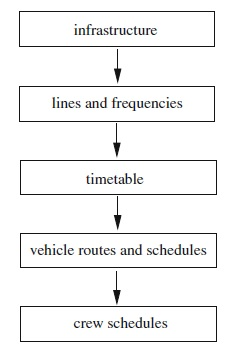
\includegraphics[width=5.5cm]{phases.jpg}% 
\caption{\small The planning steps in public transportation}
\end{figure}
This means that different problems arise in public transport: 
\begin{itemize}
\item \emph{network design} deals with the layout of the transportation system. Decision are made about choosing streets/providing tracks of sufficient capacity to support the passengers' demand such that construction costs are minimized. The general design of a transit network is the highest level activity, undertaken only rarely or when major new system (e.g. rail or express bus) are introduced;
\item given the infrastuctural data, the \emph{line planning problem} consists of finding a line concept that specifies the paths and frequencies;
\item the problem of \emph{timetabling} that is to specify arrival and departure times of trains and buses  in a timetable; and
\item the problem of \emph{delay management} whose task is, given an operating public transportation system and a set of delays occurring in the daily operations, to decide whether trains should wait for delayed trains and buses or depart on time and to update the existing timetable to incorporate this changes.
\end{itemize}
Since public transportation problems are often very complex and hard to solve, most works concentrate only on one problem at a time, although there exist some attempts to combine multiple problems identified in public transportation planning into one large model. \newline
As mentioned before, there are two conflicting goals when determing a line concept. On the one hand, the line concept should be as good as possible for the passengers and, on the other hand, the costs for setting up and running the transit system should be small. Consequently, there are cost- and passengers- oriented components in all models for the line planning problem. We will call a model \emph{passenger-oriented} if its objective is to maximize the quality of the line concept (costs may be restricted in the constraints). Analogously, a model in which the goal is to minimize the costs while the constraints ensure a minimum level of quality for the passengers will be called \emph{cost-oriented}. \newline
We are interested in modeling the quality for the passenger. \newline
First, we have to observe that between different passenger-oriented line planning models there is one crucial difference. \newline
Up to the beginning of this century, mathematical line planning models used a given Origin-Destination-matrix only to distribute the passengers on paths in the transportation network before the lines where known. This first step is known as \emph{traffic assignment} and generates the traffic loads by routing passengers through the public transportation network along suitable paths. In  a second step there is the actual planning of lines, timetabling, etc. \newline
However, the real passengers' weights along every edge strongly depend on the line concept which is to be designed, leading to a chicken-egg-problem. \newline
Hence, a great challenge is the integration of line planning and passenger routing, and this is a central topic of the thesis. \newline
Moreover, we have to remind that an important step when approaching an optimization problem, in particular if real-world instances can be expected to be large, is to investigate the complexity of the problem. For this reason we studied the complexity of the problem and we identify classes of istance  for which the problem can be solved in polynomial or pseudopolynomial time.



\chapter{State of the art}
This section provides a short overview of the literature  for the line-planning problem. The line planning problem has been investigate extensively in the operations research literature over last forty years. We are going to consider separately the literature on the cost-oriented and on the passengers-oriented models.
\section{Cost-oriented models}
Most of literature about line planning in public transport is about the cost-oriented models. \newline
In the literature it is common to work in two step approaches. These approaches precompute some set of lines in a first phase and choose a line plan from this set in a second phase. For example, Ceder and Wilson \cite{ceder:art} described an enumeration method to generate lines whose length is within a certain factor from the length of the shortest path, while Mandl \cite{mandl:art}proposed a local search strategy to optimize over such a set. \newline
An important line of developments is based on the concept of the so called \emph{system split}. Its starting points is a classification of the links of a transportation system into levels of different speed. Assuming that travelers are likely to change to fast levels as early and leave them as late as possible, the passengers are distributed onto several paths in the system - using Kirchhoff-like rules at the transit points - before any lines are known. This fixes the passenger flow on each individual link into the network. The system split was promoted by Buma and Oltrogge\cite{BoumaOltrogge:art}, who used it to develop a branch-and-bound-based software system for the planning and analysis of the line system of the Dutch railway network.
Extensive research on cost-oriented models is presented by Claessens et al. \cite{clae:art}. The goal of this work was to determines lines that minimize the operational costs subject to service constraints and capacity requirements. The (railway) model presented in Claessens et al. determines not only the lines and their frequencies, but also the type of train operating a line and the number of cars for each train. The cost investigated include fixed costs per car per hour (e.g. cost of capital, fixed maintenance), variable cost per car per kilometer (as energy costs, cleaning costs, ...), and variable costs per train per kilometer (e.g. for the driver and for energy). In this work is presented a nonlinear formulation with decision variables X$^{tc}_l$ which are defined to be one, if line l is served by vehicles of type t which c cars. The model is then linearized by increasing its dimension. The algorithm suggested uses a \emph{branch and bound procedure}\footnote{A branch and bound algorithm consists of  a systematic enumeration of candidate solutions by means of state space search: the set of candidate solution is thought as forming a rooted tree with the full set at the root. The algorithm explores branches of this tree, which represent subsets of the solution set. Before enumerating the candidate solution, the branch is checked against upper and lower estimated bounds on the optimal solution, and is discarede if it not cannot produce a better solution than the best one found so far by the algorithm.}. \newline
From this work, Goossens et al.\cite{gooss:book} proposed a \emph{branch and cut} approach\footnote{Branch and cut is a method of combinatorial optimization for solving integer linear programs. This procedure involves running a branch and bound algorithm and using cutting planes to tighten the linear programming relaxations.} to solve the line planning. Goossens investigates a probem extension called \emph{multi-line planning problem} in which not all trains need to stop at all stations. The problem is modeled as a multi-commodity flow problem, with a flow for eah type of train. A numerical analysis of the results obtained for real-world instances show that its solution is better than the solutionn obtained from solving a sequence of single-type line planning probems. \newline
In the cost-oriented model proposed by Torres et al.\cite{torres:art}, a sum of fixed and variable costs is to be minimized and only lower edge frequency requirements are present. As a generalization, the authors allow that fast lines need not stop at all stations. It is shown that the model is NP-hard even for simple network (unless restriction on costs, fleet and lines). Neverthless, the numerical results indicate that problems whose uderlyng public transportation network has a simple structure can be solved by an IP solver in reasonably time.

\section{Passenger-oriented models}
In passengers-oriented model we can distinguish two different approaches:
\begin{itemize}
\item direct travelers approach
\item traveling time approach
\end{itemize}.
The maximization of the number of direct travelers was the focus of many of the early research papers. The first formulation of direct -traveler as an integer program is given in Dienst\cite{dien:book}. The solution method proposed in this work is a branch and bound approach which builds a line partition by adding lines one after another. As next node in the branch and bound tree the line with the maximal current direct travelers is chosen in a greedy manner. In successive works, Bussieck et al. added a capacity constraints to the model. This constraints ensures that all the direct travel can be transported. The resulting models are formulated as integer programs and solved by integer programming techniques. \newline
The first integer programming approach which includes routing of passengers while minimizing the traveling time was presented in Sch\"{o}bel and Scholl \cite{schsch:art}. The goal is to design the lines in such a way that the sum of all traveling times of all passenger is minimal, respecting a budget constraint. Note that the budget constraint is crucial: otherwise, one would establish direct lines (or the shortest ossibility that can be achieved using the lines from the line pool) for any passenger. \newline
Also Bornd\"{o}rfer and Pfetsch and Bornd\"{o}rfer et al. \cite{born:art} present a model in which passenger paths can be freely routed. Their objective is to minimize the riding time (neglecting the time for transfers) to which they add fixed costs and variables costs for the line system. They present two multi-commodity flow formulations. \newline
The first formulation concerns the case in which all paths are allowed as lines and is the first integer programming model in which both the passengers' path and the paths of the lines are not fixed in advance but determined within the optimization. Flow variables and for the passengers and flow variables for the lines ensure that the lines are constructed from scratch and the passengers are routed freely through the network. \newline
Their second formulation using a variable for each potential line and for each potential passener path is the basis for their \emph{branch and price approach} \footnote{The branch and price method is a hybrid of branch and bound and column generation methods}. The authors show that the resulting pricing problem is NP-hard. \newline
Another formulation also allowing the passengers to be freely routed was developed in Nachtigall and Jerosch. They consider the traveling times of all passengers including a penalty for transfers. In their formulation, they look for a combination of partial routes which significantly reduces the number of variables needed making the problem numericallly tractable. In order to minimize the traveling time, they use upper edge frequency and upper node frequency requirements, while the use a budget constraints in order to bound the costs. \newline

\section{Game-theoretic models}
For sake of completeness, we will briefly review the most important results concerning line planning problem in public transport. \newline
In order to obtain delay-resistant line plans, Sch\"{o}bel and Schwarze \cite{schbel_et_al:inpro}present a game-theoretic approach to line planning. The lines correspond to the players that decide about their frequencies. Their individual benefit functions include the delay-resistance of their lines which does depend on all line using the same infrastructure and hence on the decision of the other players. An equilibrium ensures that the frequencies are equally distributed over the network, and hence, delays due to capacity conflicts are less likely. \newline
Another game-theoretic approach has been suggested in Kontogiannis and Zaroliagis \cite{kontogiannis_et_al:inpro}. In this work, a potentially large number of line operators is given which have their lines fixed and try to maximize their personal benefits. The authors introduce a network operator whose duty is the management ofthe infrastructure. The goal of the network operatoris to achieve a social optimum by maximizing the sum of benefits of the operator. It is shown how this can be accomplished in certain situations by suggesting a pricing scheme for the usage of the shared infrastructure which is robust with respect to the different, uncertain benefit functions of the single operators.


\chapter{Modeling the Line Planning Problem}

\section{Preliminary Definition}
In this section, we will identify the basic ingredients of the Line Planning Problem.
\begin{definition}
A PTN = (V, E) is an undirected network. It represents a public tranportation network with stops (or station) V and physical connections (i.e. the tracks) E.
\end{definition}
The PTN describes the underlying street or track network we assume to be given and fixed. We assume that all lines will be operated by homogeneous vehicles, i.e., we only consider one single transport mode. In particular, we are going to consider buses. This is certainly not a realistic assumption, but nevertheless makes algorithmically sense since different modes of transport are often considered one after another.
\begin{definition}
A \textbf{line} is a path in the PTN which is served by buses. 
\begin{itemize}
\item A \textbf{one-directional line} l is given by a sequence (s$_1$, e$_1$, s$_2$, e$_2$, ..., e$_{k-1}$, s$_k$) of vertices s$_i$ $\in$ S and edges e$_i$ $\in$ E such that e$_i$ = \{s$_i$, s$_{i+1}$\} which contains every node of the PTN at most once, unless s$_1$ = s$_k$.
\item A \textbf{bi-directional line} is a sequence (s$_1$, e$_1$, s$_2$, e$_2$, ..., e$_{k-1}$, s$_k$, e$_{k-1}$, e$_2$, s$_2$, e$_1$, s$_1$) with s$_i$ $\ne$ s$_j$ for all i, j.
\end{itemize}
\end{definition}
Every line l is assigned a monotonously increasing function $\alpha_l$ : $\mathbb{R}^+_0 \rightarrow \mathbb{R}^0_+$, called \textbf{line driving time function}. \newline
Furthermore, every line is assigned a line cost $\beta_l$ which specifies the cost caused by establishing line l with frequency f$_l$. The line cost $\beta_l$ consists of a fixed cost $\kappa$ $\ge$ 0 and a per-bus cost b$_l$ $>$ 0, i.e. $\beta_l$(f$_l$) = b$_l$f$_l$ + $\kappa_l$. \newline
We denote by:
\begin{itemize}
\item S(l) := \{s $\in$ S: s $\in$ l\} the stations visited by line l
\item E(l) := \{e $\in$ E: e $\in$ l\} the edges visited by line l
\item $\mathcal{L}$(s) := \{l: l $\ni$ s\} the lines visiting a given station s
\item $\mathcal{L}$(e) := \{l: l $\ni$ e\} the lines visiting a given edge e
\end{itemize}
\begin{definition}
A \textbf{line pool} $\mathcal{L}$ is a set of lines from which the lines can be choosen.
\end{definition}
\begin{definition}
The \textbf{frequency} f$_l$ $\in$ $\mathbb{N}$ of a line l says how often service is offered along line l within a given time period. 
\end{definition}
In capacited line planning, a \textbf{line concept} is  set $\mathcal{L'}$ $\subset$ $\mathcal{L}$ together with a frequency f$_l$  $\in$ $\mathbb{N}$ for every l $\in$ $\mathcal{L'}$. Since in uncapacited line planning the frequencies are either 0 (the line is not contained in the line concept) or 1 (the line is contained in the line concept), we often omit stating the frequencies explicitly and call $\mathcal{L'}$ a line concept. \newline
We assume an overall budget B on the costs of a line concept. That is, a line concept $\mathcal{L'}$ $\subset$ $\mathcal{L}$ is \textbf{feasible} if $\sum_{l\in\mathcal{L'}}$ $\beta_l$ $\le$ B. \newline 
The passengers' demand for traveling between the station is given by the OD-pairs set.
\begin{definition}
A set of \textbf{OD-pairs} is a subset of pairs of stations $\mathcal{OD}$ = \{(u$_i$, v$_i$): i = 1,...,m\} $\subset$ S $\times$ S. There is a weight w$_{uv}$ assigned to each OD-pair representing the number of passengers who want to travel from s(u) to s(v).
\end{definition}
In order to describe a passenger's journey, we now introduce the following important definition.
\begin{definition}
A \textbf{line-route} P$_{uv}$ for a passenger of OD-pair (u, v) $\in$ $\mathcal{OD}$ specifies
\begin{itemize}
\item a path P = (s$_1$, e$_1$, s$_2$, e$_2$, ..., e$_{j-1}$, s$_j$) with s$_1$ := u and s$_j$ := v
\item for each edge e$_i$ $\in$ P a line l $\in$ $\mathcal{L}$(e$_i$) which is chosen for traveling on e$_i$
\end{itemize}
P is called the \textbf{path corresponding to} P$_{uv}$ in the PTN. Moreover, we say that a line-route P$_{uv}$ is \textbf{feasible} for a line concept $\mathcal{L'}$ if P$_{uv}$  uses only lines contained in $\mathcal{L'}$. Note that P$_{uv}$ does not only specify the path in the PTN, but also the lines used for traveling on the path and the stations where transfers between lines take place.
\end{definition}
The travel time along P$_{uv}$ includes the riding time and a penalty for every transfer:
\begin{equation} \notag
c(\mathcal{L'}, P) := d(\mathcal{L'}, P) + t(\mathcal{L'}, P)
\end{equation}
where
\begin{itemize}
\item d($\mathcal{L'}$, P) = $\sum_{e \in P}$ $\alpha_l$L$_e$, with L$_e$ edge lenght, is the driving time
\item t($\mathcal{L'}$, P) =  $\sum_{s \in P} p^{ll'}_s$, is the transfer time. We observe that the trasfer penalties $p^{ll'}_s$ are assumed to depend on the station s where the transfer takes place and on the lines l and l' between it is performed.
\end{itemize}
\begin{definition} A \textbf{line-routing for OD-pair (u, v)} is a set $\mathcal{R}_{uv}$:= \{P: line-route P is used by (u, v)\} that specifies a line-route for every passenger in (u, v). \newline
A \textbf{line-routing} $\mathcal{R}$ is a set which contains a line-routing for every OD-pair (u, v) $\in$ $\mathcal{OD}$:
\begin{equation} \notag
\mathcal{R} := \{P_{uv} : (u, v) \in \mathcal{OD}\}
\end{equation}
\end{definition}
We denote by w$^P_{uv}$ the number of passengers of OD-pair (u, v) using the line route P and require that $\sum_{P \in \mathcal{R}_{uv}}$ w$^P_{uv}$ = w$_{uv}$. In uncapacited line planning we assume that all passengers of an OD-pair take the same line-route and, in this case a line-routing is just a collection of exactly one path P$_{uv}$ for every OD-pair (u, v). \newline
A line-routing $\mathcal{R}$ is \emph{feasible for a given line concept} $\mathcal{L'}$ if every line-route in $\mathcal{R}$ is feasible for $\mathcal{L'}$ . \newline
On the other hand, a line concept $\mathcal{L'}$ is \emph{feasible for a line-routing} $\mathcal{R}$ if it is a feasible line-concept, if all lines used by $\mathcal{R}$ are contained in $\mathcal{L'}$. \newline
Obviously both these definitions require additional constraints in case of capacity restrictions. \newline
Let $\mathcal{L'}$ be a line concept and $\mathcal{R}$ a line-routing. The \emph{overall travel time} is defined as
\begin{equation} \notag
c(\mathcal{L'}, \mathcal{R}) := \sum_{(u, v) \in \mathcal{OD}} \sum_{P \in \mathcal{R}_{uv}} w^P_{uv}c(\mathcal{L'}, P)
\end{equation} 




\section{The Change-and-Go Network}
In order to depict the various travel possibilities from the origins to the destinations, we introduce the change-and-go network (CGN). The concept of the change-and-go network combines the PTN, the line pool and the OD-pairs into one network model. \newline 
Given a public transportation network $\mathcal{PTN}$ = (S, E), a line pool $\mathcal{L}$ and a set of OD-pairs $\mathcal{OD}$, the CGN = (V, A) is constructed in the following way. \newline
The set of nodes V is defined as
\begin{equation} \notag
V := V_{travel} \cup V_{org} \cup V_{dest}
\end{equation}
where
\begin{itemize}
\item V$_{travel}$ := \{[s, l] : s $\in$ S, l $\in$ $\mathcal{L}$(s)\} is the set of \emph{travel nodes}
\item V$_{org}$ := org($\mathcal{OD}$) = \{u$^{org}$ : (u, v) $\in$ $\mathcal{OD}$\} is the set of \emph{origin nodes}
\item V$_{dest}$ := dest($\mathcal{OD}$) := \{v$^{dest}$ : (u, v) $\in$ $\mathcal{OD}$\} is the set of \emph{destination nodes}
\end{itemize}
In these definitions, org and dest are two mapping that map an OD-pair (u, v) to an \emph{origin node} u$^{org}$ := org(u, v) and to a \emph{destination node} v$^{dest}$ := dest(u, v). \newline
The edge set A is defined as
\begin{equation} \notag
A := A_{drive} \cup A_{trans} \cup A_{org} \cup A_{dest}
\end{equation}
where
\begin{itemize}
\item A$_{drive}$ := \{([s, l], [s', l]) : l $\in$ $\mathcal{L}$, \{s, s'\} $\in$ E(l), s$\le_{l}$ s'\} $\subset$ V$_{travel}$ x V$_{travel}$ is the set of \emph{driving arcs}. The lenght of a driving arc ([s, l], [s', l]) is given as c$_{([s, l], [s', l])}$ := L$^l_{ss'}$
\item A$_{trans}$ := \{([s, l], [s, l']) : s $\in$ S, l $\ne$ l' $\in$ $\mathcal{L}$(s)\} $\subset$ V$_{travel}$ x V$_{travel}$ is the set of \emph{tranfer arcs}. The lenght of a transfer arc ([s, l], [s, l'])  is given as c$_{([s, l], [s, l'])}$ := p$^{ll'}_s$
\item A$_{org}$ := \{(u$^{org}$, [u, l]) : u$^{org}$ $\in$  V$_{org}$, [u, l] $\in$ V$_{travel}$\} is the set of \emph{origin arcs} $\subset$ V$_{org}$ x V$_{travel}$. The lenght of every origin arc (u$^{org}$, [u, l]) is set to c$_{(u^{org}, [u, l])}$ := 0
\item A$_{org}$ := \{([v, l], v$^{dest}$) : v$^{dest}$ $\in$  V$_{dest}$, [v, l] $\in$ V$_{travel}$\} is the set of \emph{destination arcs} $\subset$ V$_{travel}$ x V$_{dest}$. The lenght of every destination arc ([v, l], v$^{dest}$) is set to c$_{([v, l], v^{dest})}$ := 0
\end{itemize} 
The following is an example on the construction of the CGN.\newline
\begin{figure}[htbp]
\centering
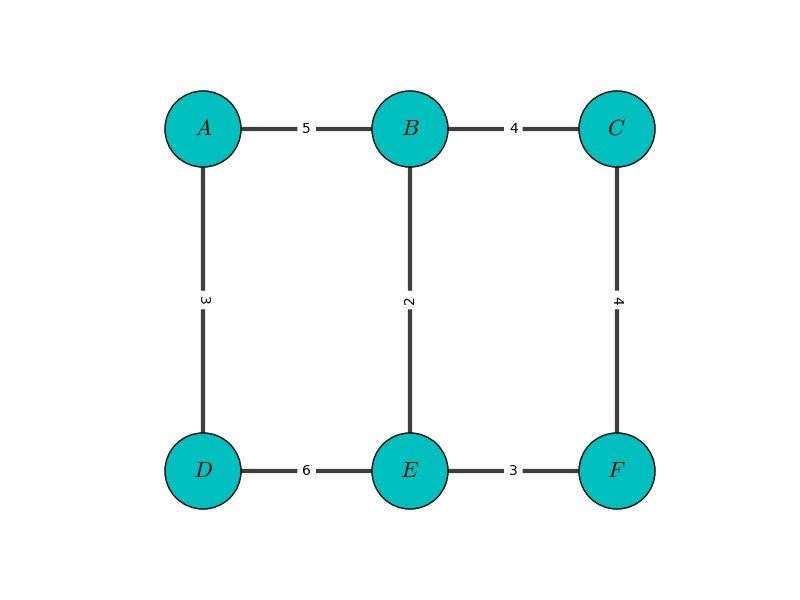
\includegraphics[width=11cm]{esempio1.jpeg}% 
\caption*{Figure 1: Public transportation network}
\end{figure}
In Figure 1 is depicted the public transportation network. The nodes represent stations, the edges represent possible direct rides.\newline
The line pool is $\mathcal{L}$ = \{l$_1$ : A - B - C, l$_2$ : D - E - F, l$_3$: A - D - E - B - A, l$_4$: C - F\} with line-driving time $\alpha_{l_1}$(x) := $\frac{1}{2}$x, $\alpha_{l_2}$(x) := $\frac{1}{3}$x, $\alpha_{l_3}$(x) := x and $\alpha_{l_4}$ := $\frac{5}{4}$x. The OD-pairs are (A, F) and (D, C). \newline
In Figure 2 the CGN is shown. The yellow lines represent the origins and destinations of the passengers and the green lines stand for the transfer possibilities between two lines.
\begin{figure}[htbp]
\centering
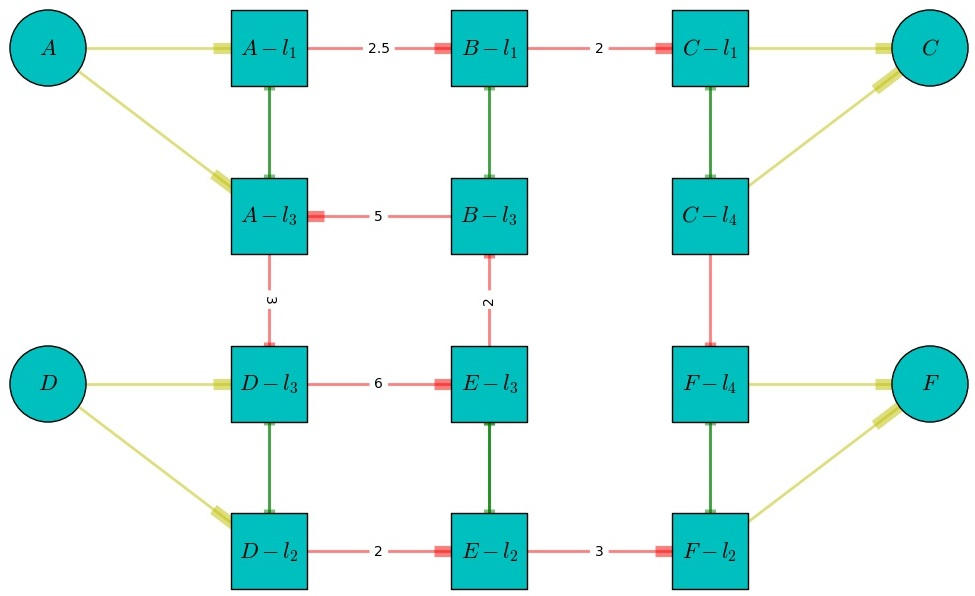
\includegraphics[width=12cm]{figura1.jpg}% 
\caption*{Figure 2: Constructed change\&go network}
\end{figure}
\begin{definition} Given a line concept $\mathcal{L}$', the network obtained by removing all arcs belonging to the lines in $\mathcal{L}\setminus\mathcal{L}$' is called \textbf{routing newtork}.
\end{definition}
Let be $\mathcal{L}$' be a line concept and P a path in the routing network N($\mathcal{L}$). We now redefine the concept of driving time, transfer time, travel time and costs along a line route to paths in N: 
\begin{itemize}
\item d($\mathcal{L}$', P) = $\sum_{a \in P \cap A_{drive}}$ c$_a$, is the \emph{driving time along P}
\item t($\mathcal{L}'$, P) = $\sum_{a \in P \cap A_{trans}}$ c$_a$, is the \emph{transfer time along P}
\item c($\mathcal{L}'$, P) = d($\mathcal{L}$', P) + t($\mathcal{L}'$, P), is the \emph{travel time along P}
\item b($\mathcal{L}'$, P) = $\sum_{l:\exists s\in S s.t. [s,l]\in P}$ b$_l$, is the \emph{cost along P}.
\end{itemize}
If P'$_{uv}$ is a feasible line-route and P$_{uv}$ is the corresponding path in N, it holds that
\begin{equation} \notag
d(\mathcal{L}', P'_{uv}) = d(\mathcal{L}', P_{uv})
\end{equation} \notag
\begin{equation} \notag
t(\mathcal{L}', P'_{uv}) = t(\mathcal{L}', P_{uv})
\end{equation} \notag
\begin{equation} \notag
c(\mathcal{L}', P'_{uv}) = c(\mathcal{L}', P_{uv})
\end{equation}
\begin{equation} \notag
b(\mathcal{L}', P'_{uv}) = b(\mathcal{L}', P_{uv})
\end{equation}
Hence we can identify line-routes and corresponding paths in N.\newline
\begin{definition} For a given line concept $\mathcal{L}'$, a routing $\mathcal{R}$ in the routing network N$\mathcal{L}$' is a \textbf{shortest-path routing} for $\mathcal{L}$', if for every OD-pair (u, v) $\in$ $\mathcal{OD}$ the travel time on every path P $\in$ $\mathcal{R}_{uv}$ equals the transfer time on a shortest path from u$^{org}$ to v$^{dest}$ in N($\mathcal{L}$').
\end{definition}
Therefore, using the above definitions and observations, follows the concept of feasibility in the line routing notation. Infact, a routing $\mathcal{R}$ in N is \emph{feasible} for a line concept $\mathcal{l}$' if $\mathcal{R}$ is a routing in N($\mathcal{L}$'). \newline
In case of capacited linne planning, the feasiblity requires also the constraints
\begin{equation} \notag
\sum_{(u,v)\in\mathcal{OD}} \sum{P\in\mathcal{R}_{uv}:P\ni a} w^{P}_{uv} \le f_{l(a)}Cap \quad \quad \forall a \in A_{drive}
\end{equation}
That means, given a line concept $\mathcal{L}$', a routing is feasible if and only if the corresponding line-routing is feasible for $\mathcal{L}$'.



\chapter{Uncapacited Line Planning with Routing}
\begin{definition} An instance (N, $\mathcal{L}$, $\mathcal{OD}$, B) of \textbf{uncapacited line planning with routing} consists of a CGN N, a line pool $\mathcal{L}$, a set of OD pairs $\mathcal{OD}$, and a budget B. \newline
The task is to choose a feasible (in the uncapacitated sense) line concept $\mathcal{L}$' and a routing $\mathcal{R}$ in N($\mathcal{L}$), such that the overall travel time c($\mathcal{L}$', $\mathcal{R}$) of the passenger is minimized.
\end{definition}
The problem is the formalized in the following way:
\begin{equation} \notag
min \sum_{(u, v) \in \mathcal{OD}} \sum_{P \in \mathcal{R}_{uv}} w_{uv}c(\mathcal{L}', P)
\end{equation}
\begin{equation} \notag
s.t. \sum_{l \in \mathcal{L}'} b_l \le B
\end{equation}. 
In this chapter we are going to study the complexity of the Line Planning problem with routing, but first we will report the principal definition about the concept of \emph{complexity}.

\section{Computational Complexity Theory}
This section briefly reviews some important concepts and results of complexity theory which will be used in the remaining chapters.
\textbf{Computational complexity theory} is a branch of the theory of computation in theoretical computer science that focuses on classifyng computational problems according to their inherent difficulty, and relating those classes to each other. \newline
To analyze the complexity of a specific problem, we must determine the amount of resource that an algorithm requires to solve instances of the problem. \newline
A complexity class is a set of problems of related complexity. Here we resume only the definitions of the classes P, NP, NP-complete and NP-hard, but first we introduce the concept of reduction.
\begin{definition} Given two subsets A and B of $\mathbb{N}$ and a set of functions F from $\mathbb{N}$ to $\mathbb{N}$ which is closed under composition, A is called \textbf{reducible} to B under F if
\begin{equation} \notag
\exists f \in F : \forall x \in \mathbb{N}, x \in A \Leftrightarrow f(x) \in B
\end{equation}
\end{definition}
Intuitively, a problem A is reducible to a problem B if an algorithm for solving problem B efficiently (if it existed) could also be used as subroutine to solve problem A efficiently.
\begin{definition} \begin{itemize}
\item The complexity class \textbf{P}, also known as \textbf{PTIME}, contains all decision problems that can be solved by a \emph{deterministic Turing machine} using polynomial time.
\item The complexity class \textbf{NP} is the set of the decision problems wher the "yes"-instances can be accepted in polynomial time by a \emph{non-deterministic Turing machine}.
\item A decision problem H is \textbf{NP-hard} when for every problem L in NP, there is a \emph{polynomial-time reduction} from L to H.
\item A decision problem H is \textbf{NP-complete} if:
\begin{enumerate}
\item H is in NP
\item every problem in NP is reducible to H in polynomial time
\end{enumerate}
In other words, NP-complete =NP $\cup$ NP-hard.
\end{itemize}
\end{definition}
In general an optimization problem may be considered as an extension of a decision problem. For this reason the previous definitions can be extended to optimization problems.


\section{Uncapacited Line Planning in General Network}
Before modeling the line planning problem we present it as a generalization of the line connectivity problem. This is an important issue because it give a first idea of the complexity of the line planning problem.
\subsection{Line Connectivity Problem}
\begin{definition} In the \emph{line connectivity problem} (LCP) it is given an undirected graph G = (V, E), a set of terminal nodes T$\subset$ V, and a set of lines $\mathcal{L}$ (simple paths) defined on the graph G. The lines have nonnegative cost and cover all edges. The problem is to find a set of lines $\mathcal{L}$' $\subset$ $\mathcal{L}$ of minimal cost such that for each pair of distinct terminal nodes t$_1$, t$_2$ $\in$ T there exists a path from t$_1$ to t$_2$, which is completely covered by lines of $\mathcal{L}$'.
\end{definition} 
NP-hardness of this this problem can be shown by reduction from the Steiner Tree problem by defining for every edge e in the PTN, a line l$_e$ with unit cost which serves only edge e. 
\begin{definition} Given an undirected graph with positive weights on its edge and a set of terminal nodes, the \emph{Steiner tree problem} consists in finding the subgraph of minimal cost such that it covers all the terminal nodes. The optimal graph is the Steiner tree.
\end{definition}
In case of only two terminals, the STP corresponds to the problem of finding a shortest path between two nodes. Also the LCP can be solved in this case by a shortest path algorithm in an auxiliary graph. If all nodes are terminal nodes, the STP becomes the \emph{minimum spanning tree} problem which can be solved  to optimality by greedy algorithms. \newline
However, it can be shown that line connectivity is NP-hard even if all nodes of the graph are terminals and all line costs are equal using a reduction from \emph{Set Cover}.
\newline
If we neglect travel time , capacity and frequency constraints, the line planning problem reduces to LCP, namely, alla stations that are departures or destinations of a passenger trip have to be connected by lines.

\subsection{Complexity analysis}
From all the observations in the previous subsection, follows this theorem.
\begin{theorem} Finding a feasible solution to the uncapacited Line Planning problem with Routing is strongly NP-hard even if
\begin{itemize} 
\item all line cost are equal,
\item the line driving functions are equal for all lines, and
\item the transfer penalties are equal for all transfers.
\end{itemize}
\end{theorem}
Hence, there is no polynomial time solution algorithms to find a feasible solution to the problem and thus there is no algorithm which finds a solution with guaranteed quality or even an optimal one. \newline
In order to understand the border between NP-hardness and polynomially computability we will hence make restrictions on the set of OD-pairs.
\begin{theorem} Line Planning with routing is strongly NP-hard, even if
\begin{itemize} 
\item there is only one OD-pair,
\item the line driving time functions of all lines are equal,
\item there are no transfer penalties, and
\item the line costs are equalfor all lines.
\end{itemize}
\end{theorem}
We prove this result by reduction from the strongly NP-complete problem \emph{Hitting Set}. \newline
An instance (P, Q, K) of \emph{Hitting Set} consists of a set P = \{p$_1$, p$_2$, ..., p$_m$\}, a set of subsets Q = \{q$_1$, q$_2$, ..., q$_n$\} of P, and a natural number K$<|$P$|$. the question is to decide is whether there is a subset P' $\subset P$ with $|$P'$|$ $\le$ K such that every q$_j$ $\in$ Q contains at least one p$_i$ $\in$ P'.
\begin{proof} 
Let (P, Q, K) be an instance of Hitting Set with P = \{p$_1$, p$_2$, ..., p$_m$\} and Q =\{q$_1$, q$_2$, ..., q$_3$\}. We construct an instance I of uncapacited Line Planning with Routing with one OD-pair in the following way.
\begin{itemize}
\item We set the set of stations to be 
\begin{equation} \notag
\begin{split}
S := \{s_1, s_{4n+2}\} \cup \{s_{4(j-1)+2}, s_{4(j-1)+4} : j = 1, ..., n\} \\ \cup \{s^i_{4(j-1)+2}, s^j_{4(j-1)+4} : j = 1, ..., n, i = 1, ..., m\} \\ \cup \{s^i_{4(j-1)+5} : j = 1, ..., n-1, i = 1, ..., m\} \quad \quad 
\end{split}
\end{equation}
and define the set of edges of the PTN as
\begin{equation} \notag
\begin{split}
E = &\{\{s_1, s_2\}\} \\ &\cup \{\{s_{4(j-1)+2}, s_{4(j-1)+3}\}, \{\{s_{4(j-1)+3}, s_{4(j-1)+4}\}, \{s_{4(j-1)+4}, s_{4(j-1)+6}\}\\ &: \quad j = 1, ..., n\} \\ \quad &\cup \{\{s^i_{4(j-1)+2}, s^i_{4(j-1)+4}\} : j = 1, ..., n, i = 1, ..., m\} \\ &\cup \{\{s^j_{4(j-1)+4}, s^j_{4(j-1)+5}, s^i_{4(j-1)+6}\} : j = 1, ..., n-1, i = 1, ..., m\}
\end{split}
\end{equation}
We set M := 2n + 2,
\begin{equation} \notag
L_{\{s_{4(j-1)+3},s_{4(j-1)+4}\}} := M \quad for \quad j = 1,..., n, 
\end{equation}
\begin{equation} \notag
L_{\{s^i_{4(j-1)+5},s^i_{4(j-1)+6}\}} := M \quad for \quad i = 1,..., m,\quad j = 1,..., n-1.
\end{equation}
All other edge lengths are set to L$_e$ := 1.\newline
Now whenever p$_i$ $\in$ q$_j$, we identify s$^i_{4(j-1)+2}$ := s$_{4(j-1)+2}$ and s$^i_{4(j-1)+4}$ := s$_{4(j-1)+4}$.
\item We have a line l$^0$ that visits stations s$_k$ in increasing order of k. Furthermore, we have m more lines l$^1$, l$^2$, ..., l$^m$. Line l$^i$ visits stations s$^i_k$ in incresing order of k. All lines l have line drivinng functions $\alpha_l$ with $\alpha_l$(x) := x for x $\in$ $\mathbb{R}^+_0$ and cost b$_l$ := 1. We set B := K + 1.
\item We set all transfer penalties to 0.
\item Our OD-pair is (u, v) with u := s$_1$ and v := s$_{4n+2}$. 
\end{itemize}
Now we claim that if and only if there is a solution to the constructed instance of Line Planning with Routing with objective value better or equal to 2n + 1, there is a solution to the given instance (P, Q, K) of Hitting Set.
\begin{enumerate}
\item Let ($\mathcal{L}$', $\mathcal{R}$) be a solution to I with c($\mathcal{L}$', $\mathcal{R}$) $\le$ 2n + 1. Let P$_{uv}$ be the path contained in $\mathcal{R}$. No arc of length M can be contained in P$_{uv}$, because otherwise
\begin{equation} \notag
(\mathcal{L}', P_{uv}) \ge M > 2n + 1.
\end{equation}
Thus, for every j = 1, ..., n, \{[s$_{4(j-1)+4}$, l$^0$], [s$_{4(j-1)+6}$, l$^0$]\} = \{[s$_{4(j-1)+4}$, l$^0$], [s$_{4j+2}$, l$^0$]\} $\in$ P$_{uv}$ and there exists an i such that \{[s$^i_{4(j-1)+2}$, l$^i$], [s$^i_{4(j-1)+4}$, l$^i$]\} $\in$ P$_{uv}$. Furthermore \{[s$_1$, l$^0$], [s$_2$, l$^0$]\} $\in$ P$_{uv}$.
Hence, for every j = 1, ..., n there is a line l$^i$ $\in$ $\mathcal{L}$' such that a transfer from line l$^0$ to line l$^i$ is possible at station s$_{4(j-1)+2}$. In other words, for every j = 1, ..., n there is an index i with l$^i$ $\in$ $\mathcal{L}$' such that s$^i_{4(j-1)+2}$ = s$_{4(j-1)+2}$. \newline
Setting P($\mathcal{L}$') := \{p$_i$ : l$^i$ $\in$ $\mathcal{L}$'\} we obtain that for every j = 1, ..., n there is an index i with p$_i$ $\in$ q$_j$. Furthermore,
\begin{equation} \notag
|P(\mathcal{L}')| = |\mathcal{L}'| - 1 = \sum_{l \in \mathcal{L}'} b_l - 1 \le B - 1 = K.
\end{equation}
\item Let P' be a solution to (P, Q, K). We define a line-route P$_{uv}$(P') for (u, v) as follows. P$_{uv}$(P') starts in s$_1$ taking line l$^0$. For every j = 1, ..., n at station s$_{4(j-1)+2}$, P$_{uv}$(P') transfers to a line l$^i$ for whose index i p$_i$ $\in$ q$_j$ holds and goes back to l$^0$ at station s$_{4(j-1)+4}$. \newline
Then by construction c($\mathcal{L}$(P$_{uv}$(P')), P$_{uv}$(P')) = 2n + 1, and
\begin{equation} \notag
\sum_{l\in\mathcal{L}(P_{uv}(P'))} b_l \le \sum_{l\in\{l^0\}\cup\{l^i:p_i\in q_i\}} b_l \le |P'| + 1 = K + 1.
\end{equation}
\end{enumerate} 
\end{proof} 



\chapter{Solving uncapacited line planning with an extended OD-pairs set}
\section{Problem description}
In this section we assume the following situation: \newline
from a pre-existing line concept $\mathcal{L'}$, the transportation management company wants to expand the set of OD-pairs to satisfy a growing demand. \newline
The transportation company wants to satisfy the demand, but also alter the line concept $\mathcal{L'}$ as little as possible. In fact, it is often important that the established line concept is preserved so as not to jeopardize relationships with current passenger and as to avoid high costs of line concept's modification. As any changes to the transit system must be commensurate with budgetary resources, in many cases the planners are not in the position to accept the most desiderable solution and they have to prioritize any modifications in order to best use available resources. \newline
Let be $\mathcal{OD'}$ = $\mathcal{OD}\cup$\{(u$_i$, v$_i$): i=m,...,t\} the new OD-pairs set.
\begin{definition} An instance ($\mathcal{PTN}$, $\mathcal{L}$, $\mathcal{L'}$, $\mathcal{OD'}$, B') of \emph{uncapacited line planning with an extended OD-pairs set} consists of a public transportation network $\mathcal{PTN}$, a line pool $\mathcal{L}$, the line concept $\mathcal{L'}$ (i.e. the solution of the problem ($\mathcal{PTN}$, $\mathcal{L}$, $\mathcal{OD}$, B)), a set of OD-pairs $\mathcal{OD'}$ and a budget B'. \newline
The task is to choose a feasible line concept $\mathcal{L''}$ and a feasible line-routing $\mathcal{R'}$, such that the overall travel time c($\mathcal{L''}$, $\mathcal{R'}$) of the passenger is minimized while the line concept $\mathcal{L''}$ is as much similar as possible to the line concept $\mathcal{L'}$. 
\end{definition}
In order to preserve the existing line-concept without significantly decrease the quality of the service for passengers, the problem can be modeled as:
\begin{enumerate}
\item the previous line planning problem with routing, in which we are going to introduce a new line pool that take into account the new requirements
\item a bi-criteria optimization problem
\end{enumerate}
In the following sections we analyze the different approaches.
\section{First approach}
In this first approach, we want to use the objective function of the original model's formulation and model the new situation by modifing the line pool $\mathcal{L'}$. \newline
We firstly observe that, in the original problem formulation, it didn't specify how the line pool $\mathcal{L}$ is built. We can reasonably assume that the line pool is constructed by generating for each pair of terminals (s(u), s(v)) all lines whose  travel time is less than or equal to k-times the travel time of the shortest path between s(u) and s(v). \newline
In order to encourage the use of the lines already existing in $\mathcal{L'}$, we add to the line pool $\mathcal{L}$ the set of lines, $\mathcal{S}$, constructed in the following way. Let be
\begin{equation} \notag
p^l_{ij} := \eta c^l_{ij} \quad \quad \forall (i, j) \in E(l), \quad \forall l \in \mathcal{L'}
\end{equation}
where $\eta$ is a proportionality factor, 0 $\le$ $\eta$ $\le$ 1. \newline
Thus, we consider a new PTN that differs from the original only for the driving time p$^l_{ij}$ of line in $\mathcal{L'}$. The set $\mathcal{S}$ is then constructed in the same way of $\mathcal{L}$, but using the new PTN. By now, we consider as line pool the set 
\begin{equation} \notag
n\mathcal{L} = \mathcal{L} \cup \mathcal{S}
\end{equation}
Obviously, the new driving time on the edges in the lines in $\mathcal{L'}$ influence the optimization process; in fact:
\begin{itemize}
\item if 0 $\le$ $\eta$ < 1, then p$^l_{ij}$ < c$^l_{ij}$. In this case the passengers consider more time-effective use the edge in a line in the line concept $\mathcal{L'}$ than in a new line
\item if $\eta$ = 1, then p$^l_{ij}$ = c$^l_{ij}$ and the passengers correctly evaluate the driving time of the edge
\end{itemize}
We have to analyze the cost of building or modifying a line l. Let be $\delta$ the cost of building a detour from a line in $\mathcal{L'}$. Thus: 
\[b'_l=
\begin{cases}
0 &  l \in \mathcal{L'}\\
b_l & l \notin \mathcal{L'}\\
n_l\delta & E(l')\subset E(l), l'\in\mathcal{L'}
\end{cases}
\]
where n$_l$ := \#\{(i, j) : (i, j) $\in$ E(l) $\setminus$ E(l')\}. \newline
Therefore the uncapacited line planning problem with an extended OD-pairs set is a simple uncapacited line planning problem with instance ($\mathcal{PTN}$, n$\mathcal{L}$, $\mathcal{OD'}$, B'). So our objective is 
\begin{equation} \notag
min \sum_{(u,v)\in\mathcal{OD'}} w_{uv}W(s(u), s(v))
\end{equation}
\begin{equation} \notag
s.t. \sum_{l\in\mathcal{L''}} b'_l \le B'
\end{equation}
Obviously, for construction, we aspect that for the OD-pairs in $\mathcal{OD}$ will be chosen the lines in $\mathcal{L'}$, while the parameter $\eta$ and the budget B' are crucial for the re-use of the line in the previous line-concept  for the new OD-pairs.
\section{Second approach} 
The uncapacited line planning problem with an extended OD-pairs set is not only passenger-oriented, but also cost-oriented. For this reason, it can be modelized as a bi-criteria optimization problem. \newline
In this case, we had two objective functions an the problem can be stated as:
\begin{equation} \notag
min \sum_{(u,v)\in\mathcal{OD'}} w_{uv}W(s(u), s(v))
\end{equation}
\begin{equation} \notag
max \sum_{(i,j)\in E} X_{ij}
\end{equation}
\begin{equation} \notag
s.t. \sum_{l\in\mathcal{L''}} b'_l \le B'
\end{equation}
where 
\[X_{ij}=
\begin{cases}
1 & $if$ (i, j) \in $E(l) for any l$ \in \mathcal{L'} \\
0 & $otherwise$
\end{cases}
\]
and b'$_l$ is as in the first approach. \newline
However we have to remember that the multi-criteria analysis allows to achieve an acceptable compromise between the different objective pursued, but often provides solutions that ara "not objectively optimal".


\cleardoublepage
%\phantomsection
\addcontentsline{toc}{chapter}{\bibname}
\printbibliography

    
\end{document}